% Build from the repository root with: make report
% Edit the front matter here; write the paper in sections/.
% Research question, study status, and next pilot: ../docs/research_plan.md.
% Same conference style and options as the GLA_Software reference project.
\documentclass[10pt,conference,compsoc]{IEEEtran}
% Shared mathematical tools and references.
% IEEEtran controls fonts, margins, headings, title blocks, and captions.
% Keep its layout consistent with the GLA_Software reference project.

\usepackage{mathtools,amssymb,amsthm}
\usepackage{bm}

% Figures and tables use the class's native caption formatting.
\usepackage{graphicx}
\graphicspath{{figures/}}
\usepackage{booktabs}

% Compact float spacing from the reference project's preamble.
\setlength{\textfloatsep}{0.5em}
\setlength{\floatsep}{0.4em}
\setlength{\intextsep}{0.4em}
\setlength{\abovecaptionskip}{0.2em}
\setlength{\belowcaptionskip}{0em}
\raggedbottom

% Theorem-like statements share one counter within each section.
% Equations retain the continuous numbering supplied by IEEEtran.
\theoremstyle{plain}
\newtheorem{theorem}{Theorem}[section]
\newtheorem{lemma}[theorem]{Lemma}
\newtheorem{proposition}[theorem]{Proposition}
\newtheorem{corollary}[theorem]{Corollary}
\theoremstyle{definition}
\newtheorem{definition}[theorem]{Definition}
\theoremstyle{remark}
\newtheorem{remark}[theorem]{Remark}

% Add further notation commands only when they are used in the report.
\newcommand{\Prob}{\mathbb{P}}
\newcommand{\E}{\mathbb{E}}
\DeclareMathOperator{\Var}{Var}
\DeclareMathOperator{\Core}{Core}

% Writing prompts inherit the surrounding font; grey identifies unfinished text.
\usepackage{xcolor}
\definecolor{placeholdergray}{gray}{0.40}
\newcommand{\placeholder}[1]{{\color{placeholdergray}#1}}

% Numeric IEEE citations and unobtrusive, clickable cross-references.
% Load hyperref near the end, and cleveref after the theorem definitions.
\usepackage{cite}
\usepackage{url}
\usepackage[hidelinks]{hyperref}
\usepackage[nameinlink,capitalise,noabbrev]{cleveref}


% Replace these placeholders with the title and the single author's details.
% IEEEtran supplies the title and author formatting.
\title{On Finite-Size Fluctuations at the 3-Core Transition in Clustered Random Graphs}
\author{%
  \IEEEauthorblockN{[Author name]}
  \IEEEauthorblockA{[Affiliation]\\
    {[Email address]}}
}
\date{}
\hypersetup{pdftitle={[Report title]},pdfauthor={[Author name]}}

\begin{document}

% Standard IEEE conference title block and first-column abstract.
\maketitle
% Match the compact space below the title in the GLA_Software reference.
\vspace{-1.5em}
\begin{abstract}
  % Write this last: question, methods, principal evidence, and limitations.
  % Do not promise agreement with the stochastic approximation before testing it.
  \placeholder{[Abstract text.]}
\end{abstract}

\section{Introduction}
\label{sec:introduction}

% Main research question (keep consistent with ../docs/research_plan.md):
% How do finite-size fluctuations affect the emergence and size of the 3-core
% in Poisson triangle-community graphs, and to what extent can a stochastic
% saddle-node approximation predict these fluctuations compared with a
% degree-matched configuration model?
%
% Motivate substantial-core emergence and the mixture of outcomes near a
% discontinuous transition. The main aim is to understand finite-size behaviour;
% the stochastic approximation is a testable hypothesis whose failure is useful.
% Link three aspects of the same experiment: survival/window width, conditional
% core-density fluctuations, and prediction of those distributions from survival.
% State the n^(-1/2) and n^(-1/4) scales as questions, not assumed conclusions.
% Position the work against CM core/fluctuation theorems (Janson--Luczak),
% community-graph local limits, and motif-aware calculations in other ensembles.
% Distinguish established results, our cavity approximation, and new numerical
% evidence; do not claim a new universality class or a triangle fluctuation proof.
% Scope: pure triangles and CM controls. Full finite-graph warning propagation
% and larger-clique mixtures remain optional extensions, not promised results.
% End with the paper's theory -> methods -> evidence progression.
\placeholder{[Finite-size research question, motivation, and scope.]}

% Avoid leaving only a heading and two lines at the foot of the preceding column.
\Needspace{14\baselineskip}
\section{Graph models and core observables}
\label{sec:models-and-observables}

\subsection{The 3-core and its size}
\label{sec:core-and-observables}

To find the 3-core, remove every vertex with fewer than three remaining
neighbours, then repeat: vertices that initially had enough neighbours may
lose them during the deletions. A simple undirected graph $G=(V,E)$ has
vertex set $V$ and edge set $E$; edges join distinct vertices and each pair
has at most one edge.
Write $n=|V|\geq1$ for its initial number of vertices. For a subset $S\subseteq V$,
the induced subgraph $G[S]$ keeps the vertices in $S$ and every edge of $G$
between them. Let $d_{G[S]}(v)$ count the neighbours of $v$ in this subgraph.
The simultaneous deletion rounds are
\begin{equation}
  S_0=V,\qquad
  S_{t+1}=\{v\in S_t:d_{G[S_t]}(v)\geq3\},
  \label{eq:core-pruning}
\end{equation}
where $t=0,1,\ldots$ counts rounds. The sets decrease and eventually stop
changing. If $S_\infty$ is the final set, then
$C_3(G)=G[S_\infty]$ is the 3-core~\cite{janson2007kcore}.

This procedure gives the unique largest induced subgraph with minimum degree
at least three. Indeed, if $G[W]$ already has that minimum degree, none of its
vertices can be the first vertex of $W$ removed: its three neighbours in $W$
would still be present. Thus every such $W$ remains inside the final set,
which itself meets the degree condition. This also proves that deleting
eligible vertices one at a time, in any order, gives the same answer.
The core may be disconnected; we count all its vertices, rather than only
its largest connected component.

The implementation uses a queue to avoid rescanning the whole graph after
each deletion. Initially queue all vertices of degree below three.
Remove the first queued vertex and its incident edges, update the degrees
of its remaining neighbours, and queue a neighbour when its degree falls
from three to two. Stop when the queue is empty. Each vertex is queued at
most once, giving work proportional to $|V|+|E|$.
The input graph is left unchanged. \Cref{fig:core-pruning} illustrates why a
single pass would be insufficient. For the configuration multigraph defined
in \cref{sec:configuration-model}, the same rule uses incident edge ends
instead of distinct neighbours, with the degree convention specified there.

\begin{figure}[b]
  \centering
  % Deterministic pruning example. The solid teal K_4 survives; dashed edges
% touch vertices deleted in the first two simultaneous pruning rounds.
% This source is a single-column graphic; its caption belongs in the section.
\begingroup
\definecolor{coreteal}{RGB}{33,112,117}
\definecolor{prunegray}{RGB}{150,156,160}
\definecolor{pruneorange}{RGB}{182,112,49}
\begin{tikzpicture}[
  x=1.2cm, y=1.05cm,
  vertex/.style={circle, minimum size=5.5mm, inner sep=0pt, font=\small},
  retained/.style={vertex, draw=coreteal, fill=coreteal!10, text=coreteal,
    line width=0.8pt},
  first/.style={vertex, draw=prunegray, fill=prunegray!12, text=black!75},
  second/.style={vertex, draw=pruneorange, fill=pruneorange!12,
    text=pruneorange},
  core edge/.style={draw=coreteal, line width=0.85pt},
  deleted edge/.style={draw=prunegray!85, dashed, line width=0.65pt}
]
  % Six edges on a,b,c,d form K_4, so every retained vertex has degree three.
  \coordinate (a) at (0,1);
  \coordinate (b) at (0,-0.5);
  \coordinate (c) at (1.5,1);
  \coordinate (d) at (1.5,-0.5);
  \coordinate (x) at (3,1);
  \coordinate (y) at (4.4,0.4);
  \coordinate (z) at (3.5,-0.7);
  \draw[core edge] (a)--(b)--(d)--(c)--(a);
  \draw[core edge] (a)--(d) (b)--(c);
  % Initially y,z have degree two, whereas x has degree three. Removing
  % y,z leaves x with only c,d, so x is removed in the next round.
  \draw[deleted edge] (c)--(x)--(d) (x)--(y)--(z)--(d);
  \foreach \v in {a,b,c,d} \node[retained] at (\v) {$\v$};
  \node[second] at (x) {$x$};
  \foreach \v in {y,z} \node[first] at (\v) {$\v$};
  \node[font=\footnotesize, text=coreteal] at (2.2,-1.3)
    {Remaining 3-core: $\{a,b,c,d\}$};
  \node[font=\footnotesize] at (2.2,-1.7)
    {Round 1: delete $y,z$.\quad Round 2: delete $x$.};
\end{tikzpicture}
\endgroup

  \caption{A fixed illustrative graph, not a random sample. Vertices $y,z$
    have degree two and disappear in the first simultaneous round. Vertex $x$
    initially has degree three, but loses $y$ and disappears in the second.
    The four mutually connected vertices $a,b,c,d$ form the final 3-core:
    its size is four and its fraction of the initial graph is $4/7$.}
  \label{fig:core-pruning}
\end{figure}

We use $M$ to distinguish the graph constructions defined below.
Their parameter $\lambda$ controls the mean number of memberships per vertex,
as specified in \cref{sec:triangle-model,sec:configuration-model}.
Let $G_{n,M}(\lambda)$ be the random input graph and define
\begin{equation}
  \begin{split}
    N_{n,M}(\lambda)&=|V(C_3(G_{n,M}(\lambda)))|,\\
    R_{n,M}(\lambda)&=N_{n,M}(\lambda)/n.
  \end{split}
  \label{eq:core-fraction}
\end{equation}
The denominator includes every initial vertex, including isolates.
When $n,M,\lambda$ are understood, we write simply $R$.
A core is empty if $R=0$. To separate substantial outcomes from small
nonempty cores, choose a fraction $\varepsilon_M\in(0,1]$ and set
\begin{equation}
  \begin{split}
    A_{n,M}(\lambda)&=\{R_{n,M}(\lambda)\geq\varepsilon_M\},\\
    p_{n,M}(\lambda)&=\Prob(A_{n,M}(\lambda)).
  \end{split}
  \label{eq:substantial-core}
\end{equation}
Thus survival means at least $\lceil n\varepsilon_M\rceil$ vertices remain;
equality with the cutoff is included. The baseline analyses use
$\varepsilon_M=0.05$ for all three graph conventions, with $0.02$ and $0.08$
as sensitivity checks in the triangle comparison. These are analysis choices
applied after pruning; they do not change the graph or its core.
At finite $n$, $0<R<\varepsilon_M$ means a nonempty core below the chosen
cutoff. A \emph{macroscopic} core instead describes growth with $n$:
its size remains a positive fraction of the input size. A single
finite-graph cutoff cannot establish that asymptotic property.

An unconditional mean or distribution includes all outcomes. The
conditional distribution keeps only substantial ones:
\begin{equation}
  F^+_{n,M}(r;\lambda)
  =\Prob\!\left(R_{n,M}(\lambda)\leq r\mid A_{n,M}(\lambda)\right),
  \label{eq:conditional-core-law}
\end{equation}
for $r\in[0,1]$, provided $p_{n,M}(\lambda)>0$.
Its mean and standard deviation describe sizes among survivors, whereas
$p_{n,M}$ describes how often they occur. The unconditional mean also
includes below-cutoff cores, which need not be empty. In an empirical
sample, estimate $p_{n,M}$ by the proportion meeting the cutoff and $F^+_{n,M}$
by the proportion of those survivors whose fractions are at most $r$.
With no survivors, conditional estimates are unavailable, not zero;
a sample standard deviation requires at least two. Existing baseline
size summaries are unconditional; conditional distributions are the separate
target of the finite-size investigation.

\subsection{Poisson triangle communities}
\label{sec:triangle-model}

A triangle community connects each of three individuals to the other two.
Combining such communities allows a vertex to belong to several triangles.
It also connects neighbours to one another, introducing the local clustering
discussed in the introduction. The construction is a triangle specialization
of random intersection graphs with communities~\cite{hofstad2021communities}.
The following specifies the finite simple graph used in the experiments.

Fix $n\geq1$ individuals, labelled $1,\ldots,n$, and a dimensionless parameter
$\lambda\geq0$. First propose independent membership counts
$\widetilde D_1,\ldots,\widetilde D_n$ with
\begin{equation}
  \Prob(\widetilde D_i=r)
  =e^{-\lambda}\frac{\lambda^r}{r!},
  \label{eq:poisson-memberships}
\end{equation}
for integers $r\geq0$. Here $\lambda$ is the mean number of membership places per individual
\emph{before conditioning}. For $\lambda=0$, every count is zero.
If the proposed total is not divisible by three, discard the entire vector
and draw again. Denote the accepted counts by $D_1,\ldots,D_n$ and their
total by $L=\sum_iD_i$. They have the joint Poisson law conditioned on
$L\equiv0\pmod3$. They are therefore not exactly independent Poisson variables
at finite $n$, and their marginal mean need not be exactly $\lambda$.
No single count is corrected and no leftover memberships are discarded.
The implementation aborts with an error after $100\,000$ unsuccessful
proposals; it never substitutes a different construction.

There are now $m=L/3$ communities, each with three labelled places.
To assign individuals to them:
\begin{enumerate}
  \item Make $D_i$ distinct membership tokens labelled $i$ for each
    individual $i$. Such a token, often called a membership stub,
    represents one place still to be assigned.
  \item Uniformly shuffle the $L$ tokens. Fill the three places of community
    one with the first three tokens, community two with the next three,
    and so on. Thus every matching of labelled tokens to labelled places
    has the same probability.
  \item In each triple, join every pair of distinct individuals, adding an
    edge only if that pair is not already connected.
\end{enumerate}
If $L=0$, there are no communities or edges, but all $n$ vertices remain.
Uniformity applies to token assignments, not to the resulting simple graphs.

The grouping does not require three different individuals. For example,
$(i,i,j)$ creates only the edge $\{i,j\}$, while $(i,i,i)$ creates none.
Repeated triples are also allowed. A connection from a vertex to itself
is omitted, and every repeated edge is merged into one, both within and
between communities. This conversion from membership places to edges is the
simple-graph \emph{projection}; the unmerged membership records are retained.
\Cref{fig:triangle-construction} shows both overlap and repeated places.
Equivalently, one can draw an incidence graph with one type of vertex for
individuals and another for communities, joining them once per assigned
place. Repeated memberships give repeated incidence edges. Core pruning is
performed on the projected graph of individuals, not on this incidence
graph, and does not require a prescribed number of whole triangles to survive.

\begin{figure}[b]
  \centering
  % Three prescribed groups of slots illustrate projection onto a simple graph.
% Two groups yield overlapping triangles. The repeated a in the third group
% contributes neither a loop nor a second copy of the already present edge ab.
\begingroup
\definecolor{motifteal}{RGB}{33,112,117}
\definecolor{slotgray}{RGB}{105,113,118}
\definecolor{slotorange}{RGB}{182,112,49}
\begin{tikzpicture}[
  x=1.15cm, y=1cm,
  vertex/.style={circle, minimum size=5.5mm, inner sep=0pt, font=\small,
    draw=motifteal, fill=white, text=motifteal, line width=0.8pt},
  slot group/.style={rectangle, rounded corners=2pt, minimum width=1.35cm,
    minimum height=5.5mm, inner sep=3pt, font=\small,
    draw=slotgray!70, fill=slotgray!5},
  edge/.style={draw=motifteal, line width=0.85pt}
]
  \node[font=\footnotesize] at (0,1.55) {Slot groups};
  \node[slot group] at (0,1) {$(a,b,c)$};
  \node[slot group] at (0,0.25) {$(c,d,e)$};
  \node[slot group, draw=slotorange, fill=slotorange!8] at (0,-0.5)
    {$(a,a,b)$};
  \draw[->, draw=slotgray, line width=0.8pt] (0.8,0.3)--(1.6,0.3);
  \node[font=\footnotesize] at (3.3,1.55) {Simple graph};
  % The resulting edge set is {ab,ac,bc,cd,ce,de}; c is shared.
  \coordinate (a) at (2.1,1);
  \coordinate (b) at (2.1,-0.5);
  \coordinate (c) at (3.4,0.25);
  \coordinate (d) at (4.7,1);
  \coordinate (e) at (4.7,-0.5);
  \fill[motifteal!7] (a)--(b)--(c)--cycle;
  \fill[motifteal!7] (c)--(d)--(e)--cycle;
  \draw[edge] (a)--(b)--(c)--cycle (c)--(d)--(e)--cycle;
  \foreach \v in {a,b,c,d,e} \node[vertex] at (\v) {$\v$};
  \node[font=\footnotesize, text=slotorange, align=center] at (2.05,-1.2)
    {The repeated $a$ adds no loop;\\$ab$ is already present.};
\end{tikzpicture}
\endgroup

  \caption{A fixed membership assignment and its simple projection.
    The triples $(a,b,c)$ and $(c,d,e)$ create two triangles sharing $c$.
    The triple $(a,a,b)$ creates no loop and adds no extra copy of $ab$.
    Membership counts are $(D_a,D_b,D_c,D_d,D_e)=(3,2,2,1,1)$, whereas
    distinct-neighbour degrees are $(2,2,4,2,2)$. This is an illustration
    of the construction, not a simulated realization.}
  \label{fig:triangle-construction}
\end{figure}

Each membership offers two edge ends, so write $K_i=2D_i$ for the
\emph{nominal} degree, before loops and repeated edges are removed.
If $\kappa_i$ is the actual number of distinct neighbours after projection,
then exactly
\begin{equation}
  \kappa_i\leq\min\{n-1,2D_i\}.
  \label{eq:triangle-degree-bound}
\end{equation}
Even a vertex with many memberships can have fewer neighbours because
some places repeat the same individual. Actual finite degrees can be odd.

For fixed $\lambda>0$ as $n\to\infty$, the divisibility condition has a
vanishing effect on any fixed number of membership counts.
Coincidences among the neighbours of a uniformly chosen vertex also become
unlikely. Its degree therefore converges in distribution to
\begin{equation}
  \begin{gathered}
    K=2D,\qquad D\sim\operatorname{Poisson}(\lambda),\\
    \pi_{2r}:=\Prob(K=2r)=e^{-\lambda}\lambda^r/r!,\\
    \pi_{2r+1}=0,\qquad r=0,1,\ldots.
  \end{gathered}
  \label{eq:limiting-degree-law}
\end{equation}
This is the triangle case of the community degree law in
\cite[Corollary~2.9 and the erasure discussion in Section~2.4]{hofstad2021communities}.
It gives $\E[K]=2\lambda$ and $\Var(K)=4\lambda$.
In particular, it is twice a Poisson variable, rather than a Poisson variable
of mean $2\lambda$. These are limiting degree statements, not identities
for the finite projected degrees or a theorem about the final 3-core.

\subsection{The degree-matched configuration model}
\label{sec:configuration-model}

The triangle construction joins neighbours in prescribed groups. To compare
it with connections formed without those groups, give each vertex a number
of individual edge ends and randomly join the ends in pairs. This is the
configuration model (CM)~\cite[Section~2]{janson2007kcore}.
For the implemented benchmark, independently draw
$D^{\mathrm{CM}}_1,\ldots,D^{\mathrm{CM}}_n$ from
$\operatorname{Poisson}(\lambda)$ and prescribe degrees
$K^{\mathrm{CM}}_i=2D^{\mathrm{CM}}_i$.
These counts are unconditioned: the total degree is automatically even.
Thus each prescribed degree has exactly the law in
\cref{eq:limiting-degree-law}, at every $n$.

Create $K^{\mathrm{CM}}_i$ distinct edge ends, or half-edge stubs, at vertex $i$.
Uniformly shuffle all ends and pair consecutive entries. A pair labelled
$(i,j)$ becomes an undirected edge, and every end is used.
Every matching of the labelled ends is equally likely; the resulting graphs
need not be equally likely. A general prescribed sequence with odd total
degree is rejected with an error, rather than repaired. That case cannot
arise for these twice-Poisson degrees.

Two ends of the same vertex form a \emph{self-loop}. Different pairs can
join the same two vertices, forming \emph{parallel edges}. The retained
CM graph keeps all of these, so it is a multigraph. Its degree counts
incident ends: a loop contributes two and each parallel edge contributes
separately. The degree at vertex $i$ is therefore exactly $K^{\mathrm{CM}}_i$.
For core pruning, keep a list of neighbours at each vertex, repeating a
neighbour once per edge to it and listing the vertex itself twice per loop.
The length of this adjacency list is its degree. On removing a vertex, mark it absent
first, then reduce each remaining neighbour's degree once per edge to it.
Its loops affect no other vertex. Queue a neighbour when its degree
crosses from three to two. The definition and order-independence argument
in \cref{sec:core-and-observables} apply with this degree convention.
It need not mean three distinct neighbours: two vertices joined by three
parallel edges already form a multigraph 3-core.

From the \emph{same} pairing we also obtain an erased simple CM graph:
delete every loop and retain one edge per unordered pair of distinct vertices.
Prune this graph separately using distinct-neighbour degrees.
Erasing can reduce degrees and core size, and can produce odd degrees.
It is different from rejecting an entire pairing until a simple graph is
obtained; in particular, its degrees need not equal the prescribed sequence.
The retained multigraph is the direct benchmark for the CM theory in
\cref{sec:configuration-theory}. The erased version checks the finite effect
of imposing the simple-graph convention used for triangles.

In the existing comparison, triangle and CM graphs use the same $n$ and
$\lambda$, with independently generated membership vectors and matchings.
Only the retained and erased CM outcomes share a pairing.
Here \emph{degree-matched} means a common limiting degree distribution,
not equal finite degree sequences, empirical histograms, or mean degrees.
A planned additional control would use one triangle-conditioned vector $D$
for both constructions and give the CM degrees $2D_i$.
It would match nominal degrees exactly, but still not generally match the
triangle graph's projected degrees. This shared-vector control is not part
of the existing baseline, and its conditioning differs from the unconditioned
CM sampler above.

To record finite departures from the common limiting law, let $\kappa_i$ be
the degree of vertex $i$ in the graph being measured: incident ends for the
retained CM and distinct neighbours for either simple graph.
The broad comparison computes all these degrees, including zeros.
It saves their histogram, mean, and population variance:
\begin{equation}
  \begin{split}
    H(j)&=\#\{i:\kappa_i=j\},\qquad j=0,1,\ldots,\\
    \bar\kappa&=\frac1n\sum_{i=1}^n\kappa_i,\qquad
    v_\kappa=\frac1n\sum_{i=1}^n(\kappa_i-\bar\kappa)^2.
  \end{split}
  \label{eq:degree-diagnostics}
\end{equation}
It also records the fraction $\sum_{j\text{ odd}}H(j)/n$ and the nominal
mean $n^{-1}\sum_iK_i$, using the corresponding model's nominal degrees.
For either construction, let $\ell$ count loops in the edge list before
erasure and $b$ count non-loop edge copies beyond the first per vertex pair.
For triangles, this list contains the three pairs of places from each
community. Erasure loses exactly $\ell+b$ edges, reducing total degree by
$2(\ell+b)$. These diagnostics quantify projection loss.

Clustering is measured on the simple graph in all cases. If it contains
$\tau$ triangles and has distinct-neighbour degrees $s_i$, define
\begin{equation}
  \mathcal T=\frac{3\tau}{\sum_{i=1}^n\binom{s_i}{2}},
  \label{eq:simple-transitivity}
\end{equation}
with $\mathcal T=0$ when the denominator is zero.
The denominator counts pairs of neighbours about a common vertex.
Each triangle closes three such pairs, so $\mathcal T$ is their connected
fraction, called transitivity. Both CM versions share this diagnostic because
they share their simple projection; it is measured before core pruning.

This benchmark preserves the limiting number of connections per vertex
while removing the requirement that they arrive in triangle communities.
The CM can still contain triangles formed by chance. Degree matching does
not control every correlation between vertices or every dependence created
by communities. Differences between the models therefore reflect those
structural changes together, rather than identifying an effect of clustering
alone. The next section develops the respective predictions for the measured
core fractions, keeping their different theoretical justifications explicit.

\Needspace{12\baselineskip}
\section{Critical behavior and finite-size predictions}
\label{sec:theoretical-predictions}

The models in \cref{sec:models-and-observables} specify how to draw a graph.
We now ask what fraction of its vertices can remain after repeated deletion,
and how that prediction changes near the transition. There are three levels
of justification: established CM core theorems, deductions from the triangle
cavity equations, and a proposed finite-size approximation for triangles.
Keeping these separate is essential when comparing the predictions with data.

\subsection{Configuration-model equations and theorems}
\label{sec:configuration-theory}

An edge can help retain its other endpoint only if the vertex supplying that
connection has at least two further surviving connections. Imagine keeping
the receiving endpoint present while testing this condition. Let $x$ be the
probability that a directed edge supplies such support. This conditional
question is called a cavity calculation: the contribution of the receiving
edge is excluded while counting the other available connections.

Write $K$ for the limiting CM degree, with probabilities $\pi_k$ from
\cref{eq:limiting-degree-law}, and let $\mu=\E[K]=2\lambda$.
Following a uniformly chosen edge reaches a degree-$k$ vertex with probability
$k\pi_k/\mu$, because it has $k$ possible incident ends. This is the
\emph{size-biased} degree law. For fixed $\lambda>0$, a bounded neighbourhood
of the CM becomes a tree as $n$ grows. Its different outward branches are
independent in the limit. Given degree $k$, the number of other supporting
edges is therefore $\operatorname{Bin}(k-1,x)$, a binomial variable with
$k-1$ trials and success probability $x$. Consequently
\begin{equation}
  x=F_\lambda(x):=
  \sum_{k\geq1}\frac{k\pi_k}{\mu}
  \Prob\{\operatorname{Bin}(k-1,x)\geq2\}.
  \label{eq:cm-support}
\end{equation}
At a uniformly chosen vertex all $k$ incident edges are available, giving
\begin{equation}
  \mathcal R_{\mathrm{CM}}(x,\lambda)=
  \sum_{k\geq0}\pi_k\Prob\{\operatorname{Bin}(k,x)\geq3\}.
  \label{eq:cm-density-sum}
\end{equation}
The predicted density is $\rho_{\mathrm{CM}}(\lambda)=
\mathcal R_{\mathrm{CM}}(x(\lambda),\lambda)$ at the selected solution.

These sums have short closed forms. The function
$G_0(t)=\E[t^K]=\exp\{\lambda(t^2-1)\}$ encodes the degree probabilities as
its coefficients. The corresponding function after following an edge is
$G_1(t)=G_0'(t)/\mu=t\exp\{\lambda(t^2-1)\}$.
The probabilities of zero and one successes are $G_1(1-x)$ and
$xG_1'(1-x)$. Subtracting them from one gives
\begin{equation}
  F_\lambda(x)=1-e^{-\lambda x(2-x)}
  [1+2\lambda x(1-x)^2].
  \label{eq:cm-support-closed}
\end{equation}
For the density, subtract the probabilities of zero, one, and two successes
using $G_0$, $xG_0'$, and $x^2G_0''/2$:
\begin{equation}
 \begin{split}
  \mathcal R_{\mathrm{CM}}(x,\lambda)
  =1-e^{-\lambda x(2-x)}\big[&1+2\lambda x(1-x)\\
    &+\lambda x^2+2\lambda^2x^2(1-x)^2\big].
 \end{split}
 \label{eq:cm-density}
\end{equation}

The zero solution always exists. To select the solution corresponding to
pruning, start with all connections available, $x_0=1$, and repeatedly set
$x_{t+1}=F_\lambda(x_t)$. Since $F_\lambda$ is increasing, this sequence
decreases to its largest fixed point. Starting at zero would miss a
positive core. Above the critical point, the CM law of large numbers
identifies \cref{eq:cm-density} at this largest, crossing root as the
limiting core fraction; below it the fraction tends to zero
\cite[Condition~2.2 and Theorem~2.3]{janson2007kcore}.
The twice-Poisson degrees satisfy the required degree and moment conditions.
That theorem's crossing condition fails at the critical tangency, so it
does not assign a deterministic density there. Critical fluctuations require
\cref{sec:fluctuation-scales} instead. At $\lambda=0$ both models are edgeless
and their core fractions are zero.

\subsection{Joint cavity equations for triangles}
\label{sec:triangle-cavity}

The triangle graph contains short cycles even as $n$ grows. Its two
neighbours in one community are connected, so treating their edges as
independent would change the pruning problem. Instead, retain the incidence
representation from \cref{sec:triangle-model}. Its local limit is a tree
of individual and community vertices~\cite[Theorem~2.14]{hofstad2021communities}.
Independence then applies between separate outward community branches.

Following a membership reaches an individual with membership count $D^*$
weighted in proportion to its count. For $D\sim\operatorname{Poisson}(\lambda)$,
\begin{equation}
  \Prob(D^*-1=j)=\frac{(j+1)\Prob(D=j+1)}{\lambda}
  =e^{-\lambda}\frac{\lambda^j}{j!}.
  \label{eq:poisson-excess-memberships}
\end{equation}
Thus both a root and an individual reached through one community have a
Poisson number of available other communities, with mean $\lambda$.

Consider a triangle containing $v,u_1,u_2$, and temporarily keep $v$ present.
Let $S_i$ count neighbours offered to $u_i$ through other communities,
evaluated with $u_i$ itself kept available. Let $J\in\{0,1,2\}$ count how many
of $u_1,u_2$ can remain
jointly and thus supply neighbours to $v$. If both $S_i\geq1$, both remain:
each has the other two triangle vertices and an external neighbour.
If one $S_i=0$, that individual is deleted, and the other remains exactly
when its external count is at least two. All other cases give $J=0$.
This local calculation retains the edge between $u_1$ and $u_2$ throughout;
it does not demand that an entire triangle survive.

Write $q_j=\Prob(J=j)$ and $p_j=\Prob(S=j)$, where $S$ is the external
support count on one limiting branch. Independence of the two external
branches gives
\begin{equation}
  \begin{gathered}
    q_2=(1-p_0)^2,\qquad q_1=2p_0(1-p_0-p_1),\\
    q_0=1-q_1-q_2.
  \end{gathered}
  \label{eq:triangle-messages}
\end{equation}
A vertex receives a Poisson number of these messages. The counts of messages
of sizes one and two are independent Poisson variables with means
$\lambda q_1$ and $\lambda q_2$. Therefore $S$ has the distribution of
$A+2B$, where $A\sim\operatorname{Poisson}(\lambda q_1)$ and
$B\sim\operatorname{Poisson}(\lambda q_2)$ are independent. Enumerating the
ways to obtain support zero, one, or two yields
\begin{equation}
 \begin{aligned}
  p_0&=e^{-\lambda(q_1+q_2)},& p_1&=\lambda q_1p_0,\\
  p_2&=\left[\lambda q_2+\tfrac12(\lambda q_1)^2\right]p_0.
 \end{aligned}
 \label{eq:triangle-closure}
\end{equation}
Together, \cref{eq:triangle-messages,eq:triangle-closure} close the equations
in $(q_1,q_2)$. A root survives when its total support is at least three, so
\begin{equation}
  \mathcal R_\triangle(q,\lambda)=1-p_0-p_1-p_2,
  \qquad q=(q_1,q_2).
  \label{eq:triangle-density}
\end{equation}

Pruning starts with every triangle offering two neighbours, $(q_1,q_2)=(0,1)$.
Iterate the probability update from that state. The quantities that decrease
are the tails $q_1+q_2=\Prob(J\geq1)$ and $q_2=\Prob(J\geq2)$;
$q_1$ alone can increase when two supports become one. Monotonicity of the
local deletion rule makes this iteration select the largest message law in
these two tails, and hence the physical density prediction.

The calculation is exact for the stated local rule on the limiting incidence
tree. Using it for the finite graph's terminal core additionally assumes that
the large-graph limit can be combined with arbitrarily many pruning rounds.
Local convergence controls each fixed depth, and does not establish that
interchange. We call the resulting $\rho_\triangle(\lambda)$ a cavity
prediction. Motif-aware core calculations provide related context
\cite{bhat2017clustered}, but do not supply a fluctuation theorem for this
particular ensemble.

\subsection{Critical points and the saddle-node expansion}
\label{sec:transition-criteria}

A positive solution first becomes available when two solution branches meet
at a turning point, called a saddle-node. For the CM set
$\mathcal G_{\mathrm{CM}}(x,\lambda)=F_\lambda(x)-x$. Its critical point
satisfies
\begin{equation}
  F_{\lambda_c}(x_c)=x_c,\qquad
  \partial_xF_{\lambda_c}(x_c)=1.
  \label{eq:cm-criticality}
\end{equation}
For fixed $x\in(0,1)$, $F_\lambda(x)$ increases strictly with $\lambda$.
Solving $F_\lambda(x)=x$ defines a parameter curve $\Lambda(x)$ whose
interior minimum gives \cref{eq:cm-criticality}. Its parameter diverges at
both ends. Moreover $F_\lambda(x)=(3\lambda+2\lambda^2)x^2+O(x^3)$ near zero,
so a positive root cannot merge continuously with zero at finite $\lambda$.
The unique critical contact and its nonzero curvature are justified in
\cref{app:support-calculations}.

For triangles, eliminate the two message probabilities by putting
$u=p_0=e^{-z}$, $z>0$. At a fixed point,
\begin{equation}
 q_2=(1-u)^2,\qquad q_1=\frac{2u(1-u)}{1+2\lambda u^2}.
 \label{eq:triangle-scalar-messages}
\end{equation}
The remaining equation is
\begin{equation}
  \mathcal G_\triangle(z,\lambda)=H(z,\lambda)
  :=\lambda(q_1+q_2)-z=0.
  \label{eq:triangle-scalar}
\end{equation}
Its derivative $H_\lambda=(1-u)^2+2u(1-u)/(1+2\lambda u^2)^2$ is positive.
Multiplying by $1+2\lambda u^2$ gives a quadratic in $\lambda$, whose positive
root is
\begin{equation}
 \begin{split}
  \Lambda(z)&=\frac{2z}{B(z)+\sqrt{B(z)^2+8u^2(1-u)^2z}},\\
  B(z)&=1-u^2-2u^2z,\qquad u=e^{-z}.
 \end{split}
 \label{eq:triangle-parameter-curve}
\end{equation}
Every positive solution lies on this curve. At fixed $\lambda$, larger $z$
means larger values of both $q_2$ and $q_1+q_2=z/\lambda$, so the largest
$z$ root gives the pruning-selected law. The criticality equations are
$H(z_c,\lambda_c)=H_z(z_c,\lambda_c)=0$.
Since $\Lambda(z)\sim(2z)^{-1/2}$ near zero and $\Lambda(z)\sim z$ at infinity,
the first solution occurs at a positive interior minimum. The update
Jacobian at zero is $\left(\begin{smallmatrix}0&2\lambda\\0&0\end{smallmatrix}\right)$;
its eigenvalues are zero, excluding a finite-parameter merger with the zero
solution. The predicted density at onset is therefore positive.
The observed single-fold shape of the explicit triangle curve is numerically
checked; an analytic uniqueness theorem is not claimed.

For either model write $y=x$ or $z$ for its scalar coordinate and
$\mathcal R_M(y,\lambda)$ for its density map, composing
\cref{eq:triangle-scalar-messages} with \cref{eq:triangle-density} for triangles.
All derivatives below hold the other argument fixed. At the critical point
both models have
\begin{equation}
  \begin{gathered}
    \mathcal G_M=\mathcal G_{M,y}=0,\\
    \mathcal G_{M,\lambda}>0,\quad \mathcal G_{M,yy}<0,\quad
    \mathcal R_{M,y}>0.
  \end{gathered}
  \label{eq:fold-conditions}
\end{equation}
Let $\delta=\lambda-\lambda_c>0$ and $v=y-y_c$. Taylor expansion gives
\begin{equation}
 \begin{split}
  0={}&\mathcal G_{M,\lambda}\delta+\tfrac12\mathcal G_{M,yy}v^2\\
    &+O(\delta^2+|v|\delta+|v|^3).
 \end{split}
 \label{eq:fold-taylor}
\end{equation}
The larger branch consequently has
$v=b_M\sqrt\delta+O(\delta)$, where
$b_M=\sqrt{-2\mathcal G_{M,\lambda}/\mathcal G_{M,yy}}$.
Expanding the density in turn gives the required result:
\begin{equation}
 \begin{split}
  \rho_M(\lambda)&=\rho_{c,M}+a_M\sqrt{\lambda-\lambda_{c,M}}
                    +O(\lambda-\lambda_{c,M}),\\
  a_M&=\mathcal R_{M,y}
       \sqrt{-2\mathcal G_{M,\lambda}/\mathcal G_{M,yy}}.
 \end{split}
 \label{eq:density-square-root}
\end{equation}
Here $\rho_{c,M}>0$ is the positive branch's right-hand limit, distinct from
the zero solution below the threshold. The direct dependence of
$\mathcal R_M$ on $\lambda$ contributes only at order $\delta$.
Thus a coefficient derived for a message coordinate must be multiplied by
$\mathcal R_{M,y}$ before predicting a core fraction.

\begin{table}[tb]
  \centering
  \caption{Critical values and density coefficients computed from the model
    equations. The triangle row is a cavity prediction. Digits express
    numerical precision for these equations, not finite-graph accuracy.}
  \label{tab:critical-predictions}
  % Generated by notebooks/theory_comparison.ipynb; regenerate with make theory-figures.
\begin{tabular}{lrrr}
\toprule
Model & $\lambda_c$ & $\rho_c$ & $a$ \\
\midrule
CM multigraph & 1.287720 & 0.137889 & 0.317959 \\
Triangle cavity & 1.228598 & 0.081112 & 0.278553 \\
\bottomrule
\end{tabular}

\end{table}

The numerical procedure first brackets the minimum of $\Lambda$ and then
bisects its derivative, rather than reporting a grid point as the threshold.
For CM, implicit differentiation gives
$\Lambda'=(1-\partial_xF_\lambda)/(\partial_\lambda F_\lambda)$;
for triangles it gives $\Lambda'=-H_z/H_\lambda$.
Above the fold, bisection on the larger-coordinate side selects the positive
branch. Residuals in the original equations check the result.
\Cref{tab:critical-predictions} records the evaluated constants.
Analytic derivative formulas are given in \cref{app:support-calculations}.
Independent centred differences and direct branch solutions verify them:
$[\rho_M(\lambda_c+\delta)-\rho_c]/\sqrt\delta$ approaches $a_M$, while the
unscaled remainder is of order $\delta$.
\Cref{fig:theory-fold} shows both the jump and this local limit.
The near-double root magnifies roundoff at extremely small offsets, so the
checks use a sequence of resolvable offsets and derivative step sizes
(\cref{app:numerical-checks}).

\begin{figure*}[tb]
  \centering
  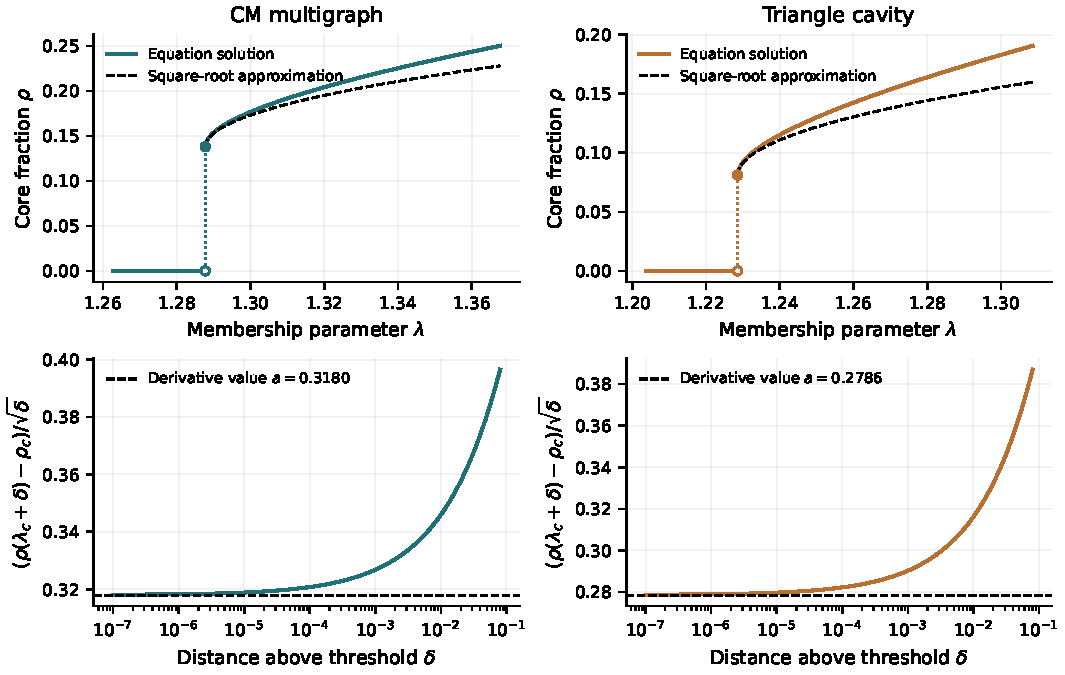
\includegraphics[width=\textwidth]{theory_fold_comparison.pdf}
  \caption{Deterministic theory near the transition. Upper panels compare the
    maximal-branch density with its leading square-root approximation. Dotted
    vertical segments indicate jumps from the separate zero branch; filled
    markers denote the positive right-hand limits. Lower panels divide the
    density increase by $\sqrt\delta$, where $\delta=\lambda-\lambda_c>0$.
    The ratios approach the derivative-based coefficients (dashed lines),
    while higher-order terms become visible farther above onset. No graph
    simulations or fitted density parameters enter this figure.}
  \label{fig:theory-fold}
\end{figure*}

\subsection{Critical windows and fluctuation scales}
\label{sec:fluctuation-scales}

Finite graphs with identical $n$ and $\lambda$ need not produce the same core.
Their sampled memberships differ, and even fixed memberships can be matched
differently. Near a turning point, a small perturbation can either leave a
positive branch available or remove it altogether. This motivates treating
the distance from criticality as a random quantity.

The CM supplies an established benchmark for this reasoning. The appropriate
results are the prescribed-degree critical theorem and the random-degree
conditioning argument of \cite[Theorem~3.5 and Section~8]{janson2008fluctuations}.
Its Erd\H{o}s--R\'enyi-specific constants cannot be used for twice-Poisson degrees.
Here is their specialization to our retained CM, with the checks and variance
calculation detailed in \cref{app:support-calculations}.

Let $\lambda_n=\lambda_c+u/\sqrt n$ for a fixed real offset $u$.
For a prescribed degree $k$, put
$h_k(x)=\E[Y\mathbf1_{\{Y\geq3\}}]$, where $Y\sim\operatorname{Bin}(k,x)$
and $\mathbf1$ is the indicator of the stated event.
In the theorem's auxiliary pruning process, the expected number of remaining
edge ends per input vertex is the mean degree times $x^2$.
The quantity $h_k(x)$ counts ends at vertices with at least three remaining
ends. Their difference counts ends at vertices still eligible for deletion.
Running out of such ends can stop the process with a positive core.
The corresponding empirical difference is
\begin{equation}
  \ell_n(x)=\frac1n\sum_{i=1}^n[K_i x^2-h_{K_i}(x)].
  \label{eq:empirical-bottleneck}
\end{equation}
Its population version is
$\ell(x,\lambda)=2\lambda x[x-F_\lambda(x)]$.
At $(x_c,\lambda_c)$ it has a quadratic minimum. Define
$c=-\partial_\lambda\ell(x_c,\lambda_c)>0$ and
$\beta=\partial_x^2\ell(x_c,\lambda_c)>0$.
The first measures the change in the minimum's height with $\lambda$;
the second measures its curvature.

Sampling the degrees makes the minimum fluctuate: if $\bar x_n$ is its
nearby minimizer, then
\begin{equation}
  \sqrt n\,\ell_n(\bar x_n)\xrightarrow{d}-cu+U,
  \qquad U\sim N(0,v_{\mathrm{degree}}).
  \label{eq:degree-noise}
\end{equation}
The pruning theorem adds an independent centred Gaussian contribution from
pairing, with variance $v_{\mathrm{pair}}$. For our degree law the two evaluated
variances are approximately $0.249099$ and $0.107879$, respectively.
Set
\begin{equation}
  \tau_{\mathrm{CM}}=
  \frac{\sqrt{v_{\mathrm{degree}}+v_{\mathrm{pair}}}}{c}
  \approx1.95625.
  \label{eq:cm-noise-scale}
\end{equation}
Let $Z\sim N(0,1)$ and $W=u+\tau_{\mathrm{CM}}Z$.
Writing $Y_{n,\mathrm{CM}}=
n^{1/4}(R_{n,\mathrm{CM}}-\rho_{c,\mathrm{CM}})$, the critical-window limits become
\begin{equation}
 \begin{split}
  \Prob(A_{n,\mathrm{CM}}(\lambda_n))
    &\longrightarrow\Phi(u/\tau_{\mathrm{CM}}),\\
  Y_{n,\mathrm{CM}}\mid A_{n,\mathrm{CM}}
    &\xrightarrow{d}a_{\mathrm{CM}}\sqrt W\mid\{W>0\}.
 \end{split}
 \label{eq:cm-critical-limit}
\end{equation}
Here $\Phi$ is the standard normal distribution function and
$\xrightarrow{d}$ denotes convergence in distribution.
Any fixed cutoff $0<\varepsilon_{\mathrm{CM}}<\rho_{c,\mathrm{CM}}$ selects
the same asymptotic substantial-core event. Both sources of randomness matter:
using pairing noise alone would give a different limit for the existing
experiments, which resample degrees on every trial.

For triangles, suppose the scalar equation has a random perturbation of
order $n^{-1/2}$ near its fold. Writing its leading noise as
$n^{-1/2}\xi$ in \cref{eq:fold-taylor} replaces $\delta$ by
$\delta+n^{-1/2}\xi/\mathcal G_{M,\lambda}$.
If the scaled perturbation has a nondegenerate limiting distribution, a
change in $\lambda$ of order $n^{-1/2}$ competes with it. The fold then turns
this into a coordinate and density displacement of order $n^{-1/4}$ on
surviving outcomes. Thus we test a window of width $O(n^{-1/2})$ and
\begin{equation}
  R_{n,M}-\rho_{c,M}=O_p(n^{-1/4})\ \text{conditional on }A_{n,M}.
  \label{eq:conditional-scaling}
\end{equation}
The notation means that $n^{1/4}(R_{n,M}-\rho_{c,M})$ stays bounded in
probability under the conditional laws. Multiplying by $n$ gives core-count
fluctuations of order $n^{3/4}$ about $n\rho_{c,M}$.
These statements apply within the critical window, not at every parameter.
Unconditionally, the distribution also contains outcomes near zero, far
from $\rho_c$. Neither the noise order nor Gaussianity follows from the
deterministic square root. They are additional triangle hypotheses;
local incidence convergence proves neither. The CM constants also do not
automatically apply to its erased projection.

\subsection{A stochastic prediction for surviving core sizes}
\label{sec:stochastic-approximation}

To obtain a prediction that can be tested without fitting the sizes it aims
to explain, let survival observations determine an effective threshold's
centre and spread. For each $n,M$, let $\mu_{n,M}$ be its centre in membership
parameter units and $w_{n,M}>0$ its width. Propose the occurrence curve
\begin{equation}
  \Prob(A_{n,M}(\lambda))\approx
  \Phi\!\left(\frac{\lambda-\mu_{n,M}}{w_{n,M}}\right).
  \label{eq:occurrence-model}
\end{equation}
This is equivalent to a normal random effective threshold. At a given
$\lambda$, abbreviate
$m=\sqrt n(\lambda-\mu_{n,M})$ and $s=\sqrt n\,w_{n,M}$, and define
\begin{equation}
  V=m+sZ,\qquad Z\sim N(0,1).
  \label{eq:random-distance}
\end{equation}
The approximation identifies survival with $V>0$. Its conditional density
prediction is
\begin{equation}
  Y:=n^{1/4}(R_{n,M}-\rho_{c,M})\mid A_{n,M}
  \ \approx\ a_M\sqrt V\mid\{V>0\}.
  \label{eq:stochastic-fold}
\end{equation}
The same random distance explains both whether a core appears and how much
its fraction exceeds the jump. Theory supplies $\rho_{c,M}$ and $a_M$;
only $\mu_{n,M},w_{n,M}$ are estimated from survival indicators.
For the CM asymptotic benchmark, $\mu_{n,\mathrm{CM}}=\lambda_c$ and
$\sqrt n\,w_{n,\mathrm{CM}}=\tau_{\mathrm{CM}}$ recover
\cref{eq:cm-critical-limit}. Allowing a finite-size centre and width makes
possible corrections measurable; their fitted values can be compared with
that limit. The width hypothesis is that $\sqrt n\,w_{n,M}$ approaches a
positive constant. Using $\lambda_c$ as the centre of the same scaled window
additionally requires $\sqrt n(\mu_{n,M}-\lambda_{c,M})$ to remain bounded.
This centre-drift condition is a separate assumption to be checked.

The model gives a full distribution, not just a mean. For $y\geq0$, its
conditional distribution function is
\begin{equation}
  F_Y(y)=1-
  \frac{\Phi\big((m-(y/a_M)^2)/s\big)}{\Phi(m/s)},
  \label{eq:stochastic-cdf}
\end{equation}
and $F_Y(y)=0$ for $y<0$. For a probability $q\in(0,1)$ its quantile is
\begin{equation}
  Q_Y(q)=a_M\sqrt{m-s\Phi^{-1}\!\big((1-q)\Phi(m/s)\big)}.
  \label{eq:stochastic-quantile}
\end{equation}
Means and variances follow by integrating this law; explicit moment formulas
are in \cref{app:support-calculations}. Convert back to a core fraction by
$R\approx\rho_{c,M}+n^{-1/4}Y$. The result is generally non-Gaussian because
it takes a square root after truncating the random distance at zero.

After the survival curve is calibrated, the conditional prediction has no
further fit parameters. Independent validation graphs then test its conditional means, standard
deviations, quantiles, and entire distribution. Complete membership vectors,
including repeated matchings or paired model outcomes from each vector, must
remain within one calibration or validation group. Calibration uncertainty
must be propagated into the predictions; conditional sizes must not be used
to adjust them. These statistical procedures belong to the next experimental
phase and are not implemented by the present deterministic calculations.

The approximation assumes that one effective threshold displacement captures
the leading size variability, that its normal occurrence model is adequate,
and that the local fold remains the relevant response. The cutoff must lie
below the positive jump. Finite graphs can have substantial core fractions
below $\rho_c$, whereas the leading law in \cref{eq:stochastic-fold} has
$Y\geq0$; persistent discrepancies there, or in spread and tails, can challenge
the approximation. Such failure is a possible result of the experiment,
not a reason to refit the conditional distribution to agree with it.

\section{Numerical methodology}
\label{sec:numerical-methodology}

% Current algorithms and baseline measurements already exist; the finite-size
% design, calibration, and held-out distribution tests below are planned.
% Keep essential assumptions and validation rules here, not only in appendices.

\subsection{Sampling, pruning, and numerical checks}
\label{sec:sampling-and-verification}
% Describe full-vector rejection and shuffled triangle slots, CM stub pairing,
% and queue-based core peeling with its stopping rule and computational cost.
% Distinguish simple-neighbour updates from multiplicity-aware CM updates;
% loops contribute twice to multigraph degree. Reuse pairings for erased controls.
% Existing 02 constructors accept fixed membership vectors and degree sequences;
% new work is experiment orchestration and recording, not another core algorithm.
% Explain scalar reduction, bracketing, maximal-root selection, fold solvers,
% residuals, tolerances, iteration limits, and checks of density derivatives.
% Compare the triangle scalar solver with full two-dimensional map iteration.
% Near-critical slowing or convergence failure is not evidence of an empty core.
% Include local-rule cases, small-graph pruning checks, independent CM formulas,
% limiting cases, finite differences, and branch/convergence cross-checks.
% Sources: 02, 05, 08; simulation patterns in 03/06/09; solver diagnostics in 10.
% Assign seeds before parallel dispatch; retain vector/matching seeds, settings,
% code version, and dataset role. UUID labels are not replay parameters.
% Give concise pseudocode if helpful, rather than notebook/class API listings.
\placeholder{[Graph algorithms, theory solvers, and reproducibility checks.]}

\subsection{Critical-window design and controls}
\label{sec:finite-size-design}
% Separate reused exploratory stages (03/04), common-setting baseline (06/07),
% and triangle-only refinement (09/10) from new allocation/calibration/validation.
% Existing 06 model streams do NOT share D; a common trial seed is not degree
% pairing. Existing 09 records cannot recover full-vector or defect diagnostics.
% Choose model-specific grids lambda=lambda_{c,M}+u/sqrt(n) for scaling.
% These generally use DIFFERENT physical lambdas and cannot be same-D pairs.
% Add a separate common-physical-lambda cohort for true shared-D comparisons;
% choose overlap with usable survivor counts and retain CM multigraph/erasure.
% Repeat independent matchings for a subset of full vectors to separate
% membership and matching variation; preserve vector IDs and actual degree data.
% Use an independent screening pilot to choose fixed calibration/validation
% budgets, precision goals, offsets, and a runtime cap; report expected and
% realised positive counts. Tail samples may be insufficient despite large totals.
% Predeclare allocation updates. Do not stop after k survivors and use ordinary
% fixed-sample intervals; adaptive allocation requires appropriate inference.
% Candidate table: sizes, offsets, physical lambdas, vectors, matching repeats,
% dataset roles, cutoff rules, and precision targets. Full settings: appendix B.
% Future label: tab:finite-size-design.
\placeholder{[Scaled grids, paired controls, and pilot-based sample planning.]}

\subsection{Survival calibration and validation}
\label{sec:calibration-and-validation}
% Fit the occurrence model using indicators only, separately by model and size.
% Keep theory-derived lambda_c, rho_c, and a_M fixed. Do not fit any conditional
% density offset, amplitude, or spread to improve prediction.
% Split calibration and validation by complete membership vector, keeping all
% repeated matchings and paired models together; avoid leakage through shared D.
% Existing inspected data are exploratory and cannot become unseen validation.
% Check the occurrence curve itself, parameter uncertainty, centre drift, and
% sensitivity to the fit range. Separate calibration from allocation screening.
% Predict conditional CDFs and summaries at held-out observations/parameter points,
% with uncertainty from the occurrence fit propagated into prediction.
% Use model controls to diagnose failure instead of recalibrating on target sizes.
% Planned schematic: theory inputs -> occurrence fit -> held-out size prediction.
\placeholder{[Indicator-only fitting, data splits, and prediction uncertainty.]}

\subsection{Distributions, uncertainty, and sensitivity}
\label{sec:distributional-analysis}
% Define survival probabilities and quantile-based window widths, then assess
% width versus n^(-1/2), with uncertainty and finite-size corrections.
% Compare unscaled and n^(1/4)-scaled conditional means, SDs, quantiles, and ECDFs
% for both models; choose a distribution discrepancy such as Wasserstein distance.
% Account for fitted occurrence parameters in goodness-of-fit calibration.
% Binomial/Wilson intervals apply to independent-vector, one-realization batches;
% repeated-vector designs need vector-cluster uncertainty, preserving model pairs.
% Bootstrap the full calibration/prediction procedure at the independent unit.
% Separate graph-to-graph spread from uncertainty of an estimated mean or SD.
% Predeclare absolute and jump-relative cutoffs. The legacy 5% event is primary;
% 2% and fractions of rho_c are sensitivity controls, while 8% nearly meets the
% predicted triangle jump and is a stress test. Flag sparse conditional samples.
% Keep thermodynamic benchmark error scores tied to their grids and excluded
% critical band. Onset brackets and smoothed slope markers are descriptive,
% not confidence intervals for lambda_c; retain only useful secondary diagnostics.
% Detailed estimation rules and supplementary sensitivity panels: appendix B.
\placeholder{[Windows, full conditional distributions, and robust uncertainty.]}

\section{Finite-size results and model comparisons}
\label{sec:numerical-results}

% Report observations here using the definitions and procedures already given.
% Copy selected plots into report/figures/; do not include every notebook export.
% Each question compares both models. The controls support those comparisons,
% rather than forming a disconnected set of notebook-by-notebook summaries.

\subsection{Limiting densities and numerical checks}
\label{sec:limiting-benchmarks}
% Compare multigraph core fractions with CM theory across sizes (07/10).
% Check limiting degree matching with histograms, moments, and odd-degree mass;
% report simple-projection transitivity and paired erasure effects.
% Distinguish sparse edge defects from their potentially large core cascades.
% Show the triangle physical branch and independent map-iteration convergence
% before using it as a density benchmark (08/10). Compare broad and focused data
% with the cavity curve, including errors away from the stated critical band.
% Compare critical parameters and right-hand jumps in a compact theory table.
% Do not imply a deterministic finite-n core at lambda_c or uniform dominance
% of either model throughout the supercritical range.
% These baseline results can reuse 07/10; density amplitudes still need checks.
% Candidate figures: theory/density overlay; branch and convergence diagnostic.
\placeholder{[Existing density benchmarks, critical values, and solver checks.]}

\subsection{Survival probabilities and window scaling}
\label{sec:survival-results}
% First connected question: observed probability curves, occurrence-model fit,
% finite-size centre drift, and widths versus n for BOTH models.
% Compare collapse in model-specific critical coordinates and give uncertainty
% on fitted scaling. Check finite-size corrections; do not assume the exponent.
% Distinguish an empirical event transition from an asymptotic threshold.
% Existing 07/10 supply exploratory outcomes; new calibrated/held-out evidence
% and width analysis are planned, not already completed.
% Candidate figures: probability/collapse panels; window-width scaling plot.
% Future labels: fig:survival-windows, fig:window-widths.
\placeholder{[Occurrence curves, centre drift, and evidence on window widths.]}

\subsection{Conditional sizes and predictive accuracy}
\label{sec:conditional-results}
% Second and third connected questions: report conditional distributions and
% compare their n^(-1/4) scale with the theory-plus-occurrence predictions.
% Show means AND SDs, quantiles, ECDFs, discrepancy measures, and uncertainty for
% both models on held-out data. Include positive counts and below-rho_c outcomes.
% The preliminary n=30000 mean/SD contrast motivates the focused pilot; its
% survival fit and prediction are not validated, saved notebook outputs.
% Do not treat a good mean or fitted survival curve as distributional agreement.
% State poor occurrence fit, poor conditional fit, and sparse-data uncertainty
% separately. A reproducible failure of the approximation is a useful result.
% Candidate figures: scaled conditional ECDF/quantile panels; mean and SD
% prediction errors with intervals. Candidate table: held-out fit diagnostics.
% Future labels: fig:conditional-distributions, tab:predictive-accuracy.
\placeholder{[Conditional size distributions and held-out prediction errors.]}

\subsection{Degree controls and sources of fluctuations}
\label{sec:controlled-comparison-results}
% Support the preceding three questions using genuinely same-D, common-lambda
% comparisons, paired CM erasure, and repeated matchings within full vectors.
% Keep these distinct from the model-specific critical-coordinate comparisons.
% Quantify membership versus matching variation, degree/projection defects,
% and sensitivity to absolute and jump-relative substantial-core thresholds.
% Use vector-level uncertainty for repeated matchings and paired contrasts.
% Existing 06 diagnostics can be reused; shared-D/nested designs are new work.
% Distinguish sparse edge defects from potentially large pruning cascades.
% Candidate panel: degree/erasure diagnostics, variance components, cutoff effects.
\placeholder{[Paired model controls, sources of spread, and sensitivity.]}

\section{Discussion}
\label{sec:discussion}

\subsection{Interpreting finite-size fluctuations}
\label{sec:structural-interpretation}
% Relate observed differences to joint support and community dependence.
% Answer what limiting degree matching controls and what it leaves uncontrolled:
% clustering is not isolated from all other correlations by this comparison.
% Bring together theorem-backed CM results, triangle predictions, and measured
% finite-size evidence without treating them as equally rigorous statements.
% Bring the three questions together: window scale, conditional fluctuation
% scale, and full distributional prediction. Explain where the approximation
% succeeds or fails and how that differs between models and graph conventions.
% Possible extra spread: membership fluctuations, matching variation, projection
% cascades, or omitted finite-size corrections. Treat explanations as hypotheses
% unless controlled evidence distinguishes them. Do not claim universality.
\placeholder{[Scaling evidence, approximation accuracy, and unexplained spread.]}

\subsection{Limitations and possible extensions}
\label{sec:limitations-and-extensions}
% Discuss finite sizes, grids, positive counts, allocation, calibration error,
% cutoff selection, model fit, and omitted higher-order terms. Distinguish
% evidence against a leading approximation from evidence against the exponents.
% Local weak convergence alone does not justify exchanging the
% graph-size and infinite-pruning-depth limits for the terminal core.
% Explain why the CM proof does not immediately cover the triangle ensemble.
% Possible future work: full factor-graph warning propagation, proof conditions,
% or larger communities. These are not completed experiments in this project.
% For K4 mixtures, separate automatic local 3-cores from a global transition.
\placeholder{[Finite-size and theoretical limitations, then scoped future work.]}

\section{Conclusion}
\label{sec:conclusion}

% Answer the introduction's questions using only results already presented.
% Address survival/window scaling, conditional fluctuations, and the independent
% predictive test together. A supported failure or an inconclusive sparse-data
% comparison is an admissible answer; agreement with the approximation is not
% a prerequisite for a meaningful finite-size investigation.
% Summarize the contribution and its evidential limits concisely.
% Do not introduce new derivations, data, or an additional research programme.
\placeholder{[Answers to the research questions and main takeaways.]}


% References are included through citations in the report text.
\bibliographystyle{IEEEtran}
\bibliography{references/refs}

% Keep essential definitions and assumptions in the main text.
% These appendices reserve space for supporting details, not new research claims.
\appendices
% Called after \appendices in main.tex; these are supporting paper sections.
% Keep core definitions, assumptions, and headline results in the main text.
\section{Supplementary derivations and checks}
\label{app:derivations-and-checks}

\subsection{Derivations and theorem assumptions}
\label{app:support-calculations}
% Reserve longer generating-function manipulations, the triangle scalar
% reduction and its admissible domain, and derivative/tangency calculations.
% Refer back to the main equations instead of giving competing definitions.
% Add longer density-derivative calculations and the CM fluctuation-theorem
% checklist: moments, nondegenerate minimum, degree-vector randomness, varying
% parameter sequences, and the effect of divisibility conditioning.
% The main text must still state the assumptions and theoretical status.
\placeholder{[Supporting algebra, density amplitudes, and theorem checks.]}

\subsection{Independent numerical and local checks}
\label{app:numerical-checks}
% Reserve detailed residual/tolerance tables, direct-iteration comparisons,
% local triangle cases, and finite-projection counterexamples where useful.
% Do not label probability-map iteration as a tested finite-graph
% warning-propagation algorithm; that larger experiment is not implemented.
\placeholder{[Supplementary solver checks and small illustrative cases.]}

\section{Experiment settings and sensitivity checks}
\label{app:experiment-details}

\subsection{Configurations and data provenance}
\label{app:configurations}
% Tabulate actual n values, lambda grids, independent repetitions, seeds,
% dataset/stage identifiers, and analysis settings used for the reported run.
% Record tolerances, critical exclusions, event cutoffs, code version, and
% reproducibility commands without reproducing configuration dictionaries.
% Separate existing exploratory runs from allocation screening, calibration,
% validation, and common-lambda paired cohorts. Record vector-level split IDs,
% matching repetitions, positive-count planning, budget caps, and allocation rules.
\placeholder{[Complete experimental settings and reproduction information.]}

\subsection{Additional diagnostics and sensitivity}
\label{app:sensitivity}
% Reserve supplementary degree/erasure panels, outcome plots, and cutoff,
% smoothing, grid, and critical-exclusion checks that support the main claims.
% Give each retained diagnostic its methodological reference and stated purpose.
% Omit unused exploratory exports instead of treating all generated files as
% necessary report figures.
% Add bootstrap/cluster details, occurrence-fit checks, goodness-of-fit
% calibration, full cutoff panels, sparse-tail counts, and secondary ECDFs.
\placeholder{[Distributional checks, uncertainty, and cutoff sensitivity.]}

\end{document}
